When initializing a neural network, the weights and biases -- which we denote collectively as the {\em parameters}\ 
of the network -- are drawn from some probability distribution. In 
the NNPDF formalism, the set of netowrk parameters at initialization for each replica is an instance 
of i.i.d. stochastic variables. The probability distribution
of the network parameters induces a probability distribution for the output of the neural networks at inizialization. 
It is well known that the probability distribution of these outputs becomes approximately gaussian when the size of
the hidden layers is increased. We call this limit the {\em large-network} limit. 
In this section, we review some basic results for the large-network limit at inizialization, and 
compare these theoretical 
predictions with the actual results obtained in numerical experiments performed with the typical networks 
used by the NNPDF collaboration. 
This preliminary study of the properties of networks at initialization also allows us to introduce the 
notation used for the networks in the rest of the paper. 

As detailed in Ref.~\cite{NNPDF:2021njg}, the NNs used for the NNPDF fit have a 2-25-20-8 architecture,
a $\tanh$ activation function,
and are initialized using a Glorot normal distribution~\cite{glorot2010understanding}. The preactivation
function of a neuron is denoted as $\phi^{(\ell)}_{i,\alpha} = \phi^{(\ell)}_i(x_\alpha)$, where $\ell$
denotes the layer of the neuron, $i$ identifies the neuron within the layer\footnote{We refer
to $i$ as the {\em neuron}\ index.}, and $x_{\alpha}$ is a point in the interval $[0,1]$.
A grid of $\ngrid=50$ points is used to compute observables in the NNPDF formalism and in this work 
we focus on the vakue of $f$ at those values of $x_\alpha$. For completeness, we list the values of $x_\alpha$ in
Tab.~\ref{tab:Xvals}.

\begin{table}[ht]
    \centering
    \begin{tabular}{|c|c|c|c|c|c|c|c|c|c|}
    \hline
    $\alpha$ & $x_\alpha$ & $\alpha$ & $x_\alpha$ & $\alpha$ & $x_\alpha$ & $\alpha$ & $x_\alpha$ & $\alpha$ & $x_\alpha$ \\
    \hline
    $1$  & $2.00 \times 10^{-7}$ & $11$ & $1.29 \times 10^{-5}$ & $21$ & $8.31 \times 10^{-4}$ & $31$ & $0.0434$ & $41$ & $0.422$ \\
    $2$  & $3.03 \times 10^{-7}$ & $12$ & $1.96 \times 10^{-5}$ & $22$ & $1.26 \times 10^{-3}$ & $32$ & $0.0605$ & $42$ & $0.480$ \\
    $3$  & $4.60 \times 10^{-7}$ & $13$ & $2.97 \times 10^{-5}$ & $23$ & $1.90 \times 10^{-3}$ & $33$ & $0.0823$ & $43$ & $0.540$ \\
    $4$  & $6.98 \times 10^{-7}$ & $14$ & $4.51 \times 10^{-5}$ & $24$ & $2.87 \times 10^{-3}$ & $34$ & $0.109$ & $44$ & $0.601$ \\
    $5$  & $1.06 \times 10^{-6}$ & $15$ & $6.84 \times 10^{-5}$ & $25$ & $4.33 \times 10^{-3}$ & $35$ & $0.141$ & $45$ & $0.665$ \\
    $6$  & $1.61 \times 10^{-6}$ & $16$ & $1.04 \times 10^{-4}$ & $26$ & $6.50 \times 10^{-3}$ & $36$ & $0.178$ & $46$ & $0.730$ \\
    $7$  & $2.44 \times 10^{-6}$ & $17$ & $1.57 \times 10^{-4}$ & $27$ & $9.70 \times 10^{-3}$ & $37$ & $0.220$ & $47$ & $0.796$ \\
    $8$  & $3.70 \times 10^{-6}$ & $18$ & $2.39 \times 10^{-4}$ & $28$ & $0.0144$ & $38$ & $0.265$ & $48$ & $0.863$ \\
    $9$  & $5.61 \times 10^{-6}$ & $19$ & $3.62 \times 10^{-4}$ & $29$ & $0.0211$ & $39$ & $0.314$ & $49$ & $0.931$ \\
    $10$ & $8.52 \times 10^{-6}$ & $20$ & $5.49 \times 10^{-4}$ & $30$ & $0.0305$ & $40$ & $0.367$ & $50$ & $1.00$ \\
    \hline
\end{tabular}

    \caption{Values of $x_\alpha$ used in the NNPDF grids for the computation of
    observables. The points are equally spaced on a logarithmic scale
    for $\alpha = 1, \ldots, XXX$, and linearly spacing for $\alpha > XXX$.
    \ac{Maybe we need to rethink the layout of this table...}
    \label{tab:Xvals}}
\end{table}

The output of the neuron identified by the pair $(\ell,i)$ is
$\rho^{(\ell)}_{i\alpha} = \tanh\left(\phi^{(\ell)}_{i\alpha}\right)$.
The parameters of the NN are the weights $w^{(\ell)_{ij}}$ and the biases $b^{(\ell)}_i$, which are
collectively denoted as $\theta_\mu$, where $\mu = 1, \ldots, P$ and the total number of parameters
is
\begin{equation}
    \label{eq:TotPar}
    P = \sum_{\ell=1}^{L} \left(n_{\ell} n_{\ell-1} + n_\ell\right)\, .
\end{equation}
The preactivation function in layer $(\ell+1)$ is a weighted average of the outputs of the neurons on 
the previous layer, namely
\begin{align}
    \label{eq:RecursionNN}
    \phi^{(\ell+1)}_{i\alpha} = \sum_{j=1}^{n_\ell} w^{(\ell+1)}_{ij} \rho^{(\ell)}_{i\alpha} + b^{(\ell+1)}_{i}\, .
\end{align}
The PDFs in the
so-called evolution basis are parametrized by the preactivation functions of the output layer $L$,
$x_\alpha f_i(x_\alpha)=A_i \phi^{(L)}_{i,\alpha}$, where $i=1, \ldots, 8$ labels the flavors.
\footnote{For simplicity, we ignore the preprocessing function $x^{-\alpha_i} (1-x)^{\beta_i}$ that
is currently used in the NNPDF fits. While the preprocessing may be useful in speeding the training
it does not affect the current discussion.}
The input layer is identified by $\ell=0$ and the activation
function for that specific layer is the identity, so that
\begin{equation}
    \label{eq:InitLayerPhi}
    \rho^{(0)}_{i,\alpha} = \phi^{(0)}_{i,\alpha} = x_{i,\alpha} =
    \begin{cases}
        x_\alpha\, , \quad &\text{for}\ i=1\, ;\\
        \log\left(x_\alpha\right)\, , \quad &\text{for}\ i=2\, .
    \end{cases}
\end{equation}
In the following we refer to the preactivation functions as {\em fields}.

The Glorot normal initialiser draws each weight and bias of the NN from independent Gaussian
distributions, denoted $p_w$ and $p_b$ respectively, centred at zero and with variances
rescaled by the number of nodes in adjacent layers,
\begin{equation}
    \label{eq:RescaledGlorotVariances}
    \frac{C^{(\ell)}_{w}}{\sqrt{n_{\ell-1} + n_{\ell}}}\, ,
    \quad \frac{C^{(\ell)}_{b}}{\sqrt{n_{\ell-1} + n_{\ell}}}\, .
\end{equation}
Following the NNPDF prescription, we have $C^{(\ell)_{w}=C^(\ell)}_{b}=1$. 
The probability distribution of the NN parameters induces a probability distribution for the
preactivations,
\begin{align}
    \label{eq:PreactAtInit}
    p\left(\phi^{(\ell)}\right)
      &= \int \mathcal{D}w\, p_w(w)\,
        \mathcal{D}b\, p_b(b)\, \prod_{i,\alpha}
        \delta\left(
          \phi^{(\ell)}_{i\alpha} - \sum_{j} w^{(\ell)}_{ij}
          \rho\left(\phi^{(\ell-1)}_{j\alpha}\right)
          - b^{(\ell)}_i
          \right)\, .
\end{align}
Note that, here and in what follows, $p(\phi^{(\ell)})$ denotes the joint probability for all the
$n_{\ell}\times\ngrid$ components of $\phi^{(\ell)}$,
\begin{align}
    \label{eq:ExplIndices}
    p\left(\phi^{(\ell)}\right) = p\left(\phi^{(\ell)}_{1,\alpha_1}, \phi^{(\ell)}_{2,\alpha_1}, \ldots,
        \phi^{(\ell)}_{n_\ell,\alpha_1}, \phi^{(\ell)}_{1,\alpha_2}, \ldots, \phi^{(\ell)}_{n_\ell,\alpha_2},
        \ldots,
        \phi^{(\ell)}_{n_\ell,\ngrid}\right)\, .
\end{align}
This duality between parameter-space and function-space provides a powerful framework to study
the behaviour of an ensemble of NNs, and in particular the symmetry properties of the distribution
$p(\phi^{(\ell)})$, see \eg~\cite{Maiti:2021fpy}. Working in parameter space, \ie\ computing the
expectation values of correlators of fields as integrals over the NN parameter, one can readily
show that
\begin{align}
    \label{eq:NeurRotInv}
    \mathbb{E}\left[
        R_{i_1j_1} \phi^{(n_\ell)}_{j_1 \alpha_1} \ldots
        R_{i_nj_n} \phi^{(n_\ell)}_{j_n \alpha_n}
    \right] =
    \mathbb{E}\left[
        \phi^{(n_\ell)}_{i_1 \alpha_1} \ldots
        \phi^{(n_\ell)}_{i_n \alpha_n}
    \right]\, ,
\end{align}
where $R$ is an orthogonal matrix in $\text{SO}(n_{\ell})$. Eq.\eqref{eq:NeurRotInv} implies
that the probability distribution in Eq.~\eqref{eq:PreactAtInit} is also invariant under rotations,
and therefore it can only be a function of $\text{SO}(n_{\ell})$ invariants. Therefore
\begin{align}
    \label{eq:PriorAction}
    p\left(\phi^{(n_\ell)}\right) =
        \frac{1}{Z^{(\ell)}} \exp\left(-S\left[\phi^{(\ell)}_{\alpha_1}
            \cdot \phi^{(\ell)}_{\alpha_2}\right]\right)\, ,
\end{align}
where
\begin{align}
    \label{eq:PhiInvariant}
    \phi^{(\ell)}_{\alpha_1}
            \cdot \phi^{(\ell)}_{\alpha_2} =
    \sum_{i=1}^{n_\ell} \phi^{(\ell)}_{i \alpha_1} \phi^{(\ell)}_{i \alpha_2}\, .
\end{align}
The action can be expanded in powers of the invariant bilinear,
\begin{align}
    \label{eq:ExpandAction}
    S\left[\phi^{(\ell)}_{\alpha_1}
            \cdot \phi^{(\ell)}_{\alpha_2}\right] =
        \frac12 \gamma^{(\ell)}_{\alpha_1\alpha_2}
            \phi^{(\ell)}_{\alpha_1} \cdot \phi^{(\ell)}_{\alpha_2} +
            \frac{1}{8 n_{\ell-1}} \gamma^{(\ell)}_{\alpha_1\alpha_2,\alpha_3\alpha_4}
            \phi^{(\ell)}_{\alpha_1} \cdot \phi^{(\ell)}_{\alpha_2} \,
            \phi^{(\ell)}_{\alpha_3} \cdot \phi^{(\ell)}_{\alpha_4} + O(1/n_{\ell-1}^2)\, ,
\end{align}
so that the probability distribution is fully determined by the couplings 
$\gamma^{(\ell)}$.\footnote{
    We have denoted {\em all}\ couplings by $\gamma^{{(\ell)}}$. Different couplings 
    are indentified by the number of indices, so that $\gamma^{(\ell)}_{\alpha_1\alpha_2}$ 
    is a two-point coupling, $\gamma^{(\ell)}_{\alpha_1\alpha_2,\alpha_3\alpha_4}$ is a four-point 
    coupling, etc. 
} 
In
Eq.~\eqref{eq:ExpandAction}, we have factored out inverse powers of $n_\ell$ for each coupling.
With this convention, and with the scaling of the parameters variances in
Eq.~\eqref{eq:RescaledGlorotVariances}, the couplings in the action are all $O(1)$
in the limit where $n_\ell\to\infty$.
As a consequence, the probability distribution at initialization is a multidimensional Gaussian at
leading order in $1/n_\ell$, with quartic corrections that are $O(1/n_\ell)$, while higher powers
of the invariant bilinear are suppressed by higher powers of the width of the layer. This power counting
defines an effective field theory, where deviations from Gaussianity can be computed in perturbation
theory to any given order in $1/n_\ell$, see \eg\ Ref.~\cite{Roberts:2021fes} for a detailed
presentation of these ideas. While the actual calculations become rapidly cumbersome, the
conceptual framework is straightforward.

At leading order, the second and fourth cumulant are respectively
\begin{align}
    &\langle \phi^{(\ell)}_{i_1,\alpha_1} \phi^{(\ell)}_{i_2,\alpha_2}\rangle
      = \delta_{i_1 i_2} K^{(\ell)}_{\alpha_1\alpha_2} + O(1/n_{\ell-1})\, , \\
    &\langle \phi^{(\ell)}_{i_1,\alpha_1} \phi^{(\ell)}_{i_2,\alpha_2}
      \phi^{(\ell)}_{i_3,\alpha_3} \phi^{(\ell)}_{i_4,\alpha_4}\rangle_c
      = O(1/n_{\ell-1})\, ,
\end{align}
where
\begin{equation}
    \label{eq:DefineKmat}
    K^{(\ell)}_{\alpha_1\alpha_2} = \left(\gamma^{(\ell)}\right)^{-1}_{\alpha_1\alpha_2}\, .
\end{equation}
The ``evolution'' of the couplings as we go deep in the NN, \ie\ the dependence of the couplings on
$\ell$, is governed by Renormalization Group (RG) equations, which preserve the power counting in
powers of $1/n_{\ell}$. At leading order,
\begin{align}
    K^{(\ell+1)}_{\alpha_1\alpha_2} &=
      \left.
      C_b^{(\ell+1)} + C_w^{(\ell+1)} \frac{1}{n_\ell}
      \langle \vec{\rho}^{\,(\ell)}_{\alpha_1} \cdot
      \vec{\rho}^{\,(\ell)}_{\alpha_2} \rangle
      \right|_{O(1)} \\
      \label{eq:RecursionForK}
      &= C_b^{(\ell+1)} + C_w^{(\ell+1)} \frac{1}{n_\ell}
      \langle \vec{\rho}^{\,(\ell)}_{\alpha_1} \cdot
      \vec{\rho}^{\,(\ell)}_{\alpha_2} \rangle_{K^{(\ell)}}\, ,
\end{align}
where
\begin{align*}
    \frac{1}{n_\ell}
      \langle \vec{\rho}^{\,(\ell)}_{\alpha_1} \cdot
      \vec{\rho}^{\,(\ell)}_{\alpha_2} \rangle_{K^{(\ell)}} =
    \int \prod_{\alpha}d\phi_\alpha\,
      \frac{e^{-\frac12 \left(K^{(\ell)}\right)^{-1}_{\beta_1\beta_2}
        \phi_{\beta_1} \phi_{\beta_2}}}
        {\left|2\pi K^{(\ell)}\right|^{1/2}}\,
        \rho(\phi_{\alpha_1}) \rho(\phi_{\alpha_2})\, .
\end{align*}
Eq.~\eqref{eq:RecursionForK} can be solved for the NNPDF architecture leading to the
covariance matrices for the output of the NNs displayed in
Figs.~\ref{Fig:KRecursionOne} and~\ref{Fig:KRecursionTwo}.
\begin{figure}[t!]
    \centering
    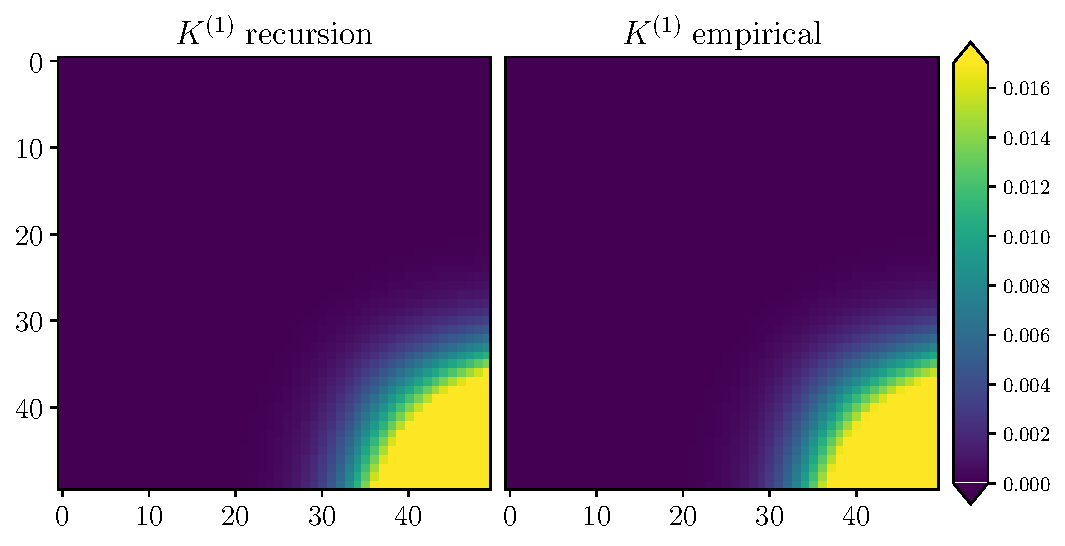
\includegraphics[scale=0.4]{figs/K1_correlations.pdf}
    \caption{The empirical (left) and analytical (right) covariance matrices $K^{(1)}$ of the first layer
    of the NNPDF architecture. The covariance in the left panel is computed ``bootstrapping'' over an
    ensemble of 100 replicas, initialised using the Glorot normal distribution. The covariance in the right
    panel is obtained by solving Eq.~\eqref{eq:RecursionForK} numerically.
    \label{Fig:KRecursionOne}
    }
\end{figure}

\begin{figure}[t!]
    \centering
    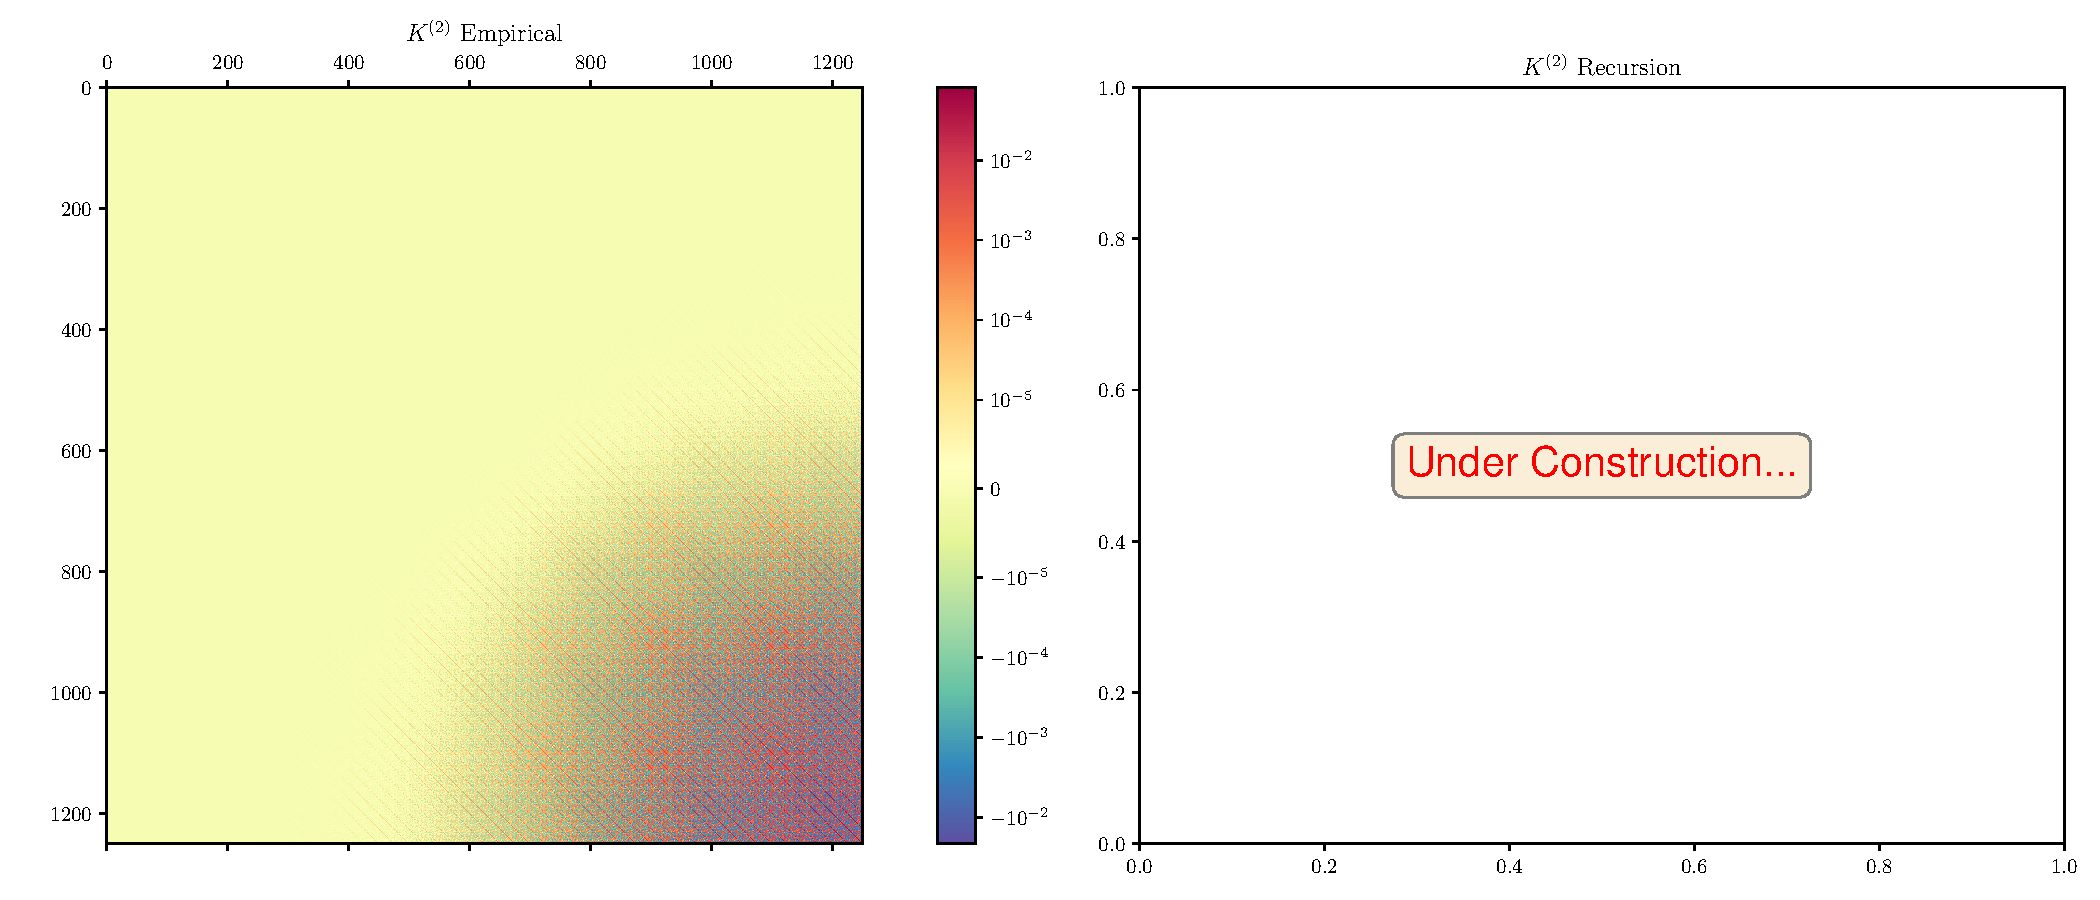
\includegraphics[scale=0.4]{figs/K2_correlations.pdf}
    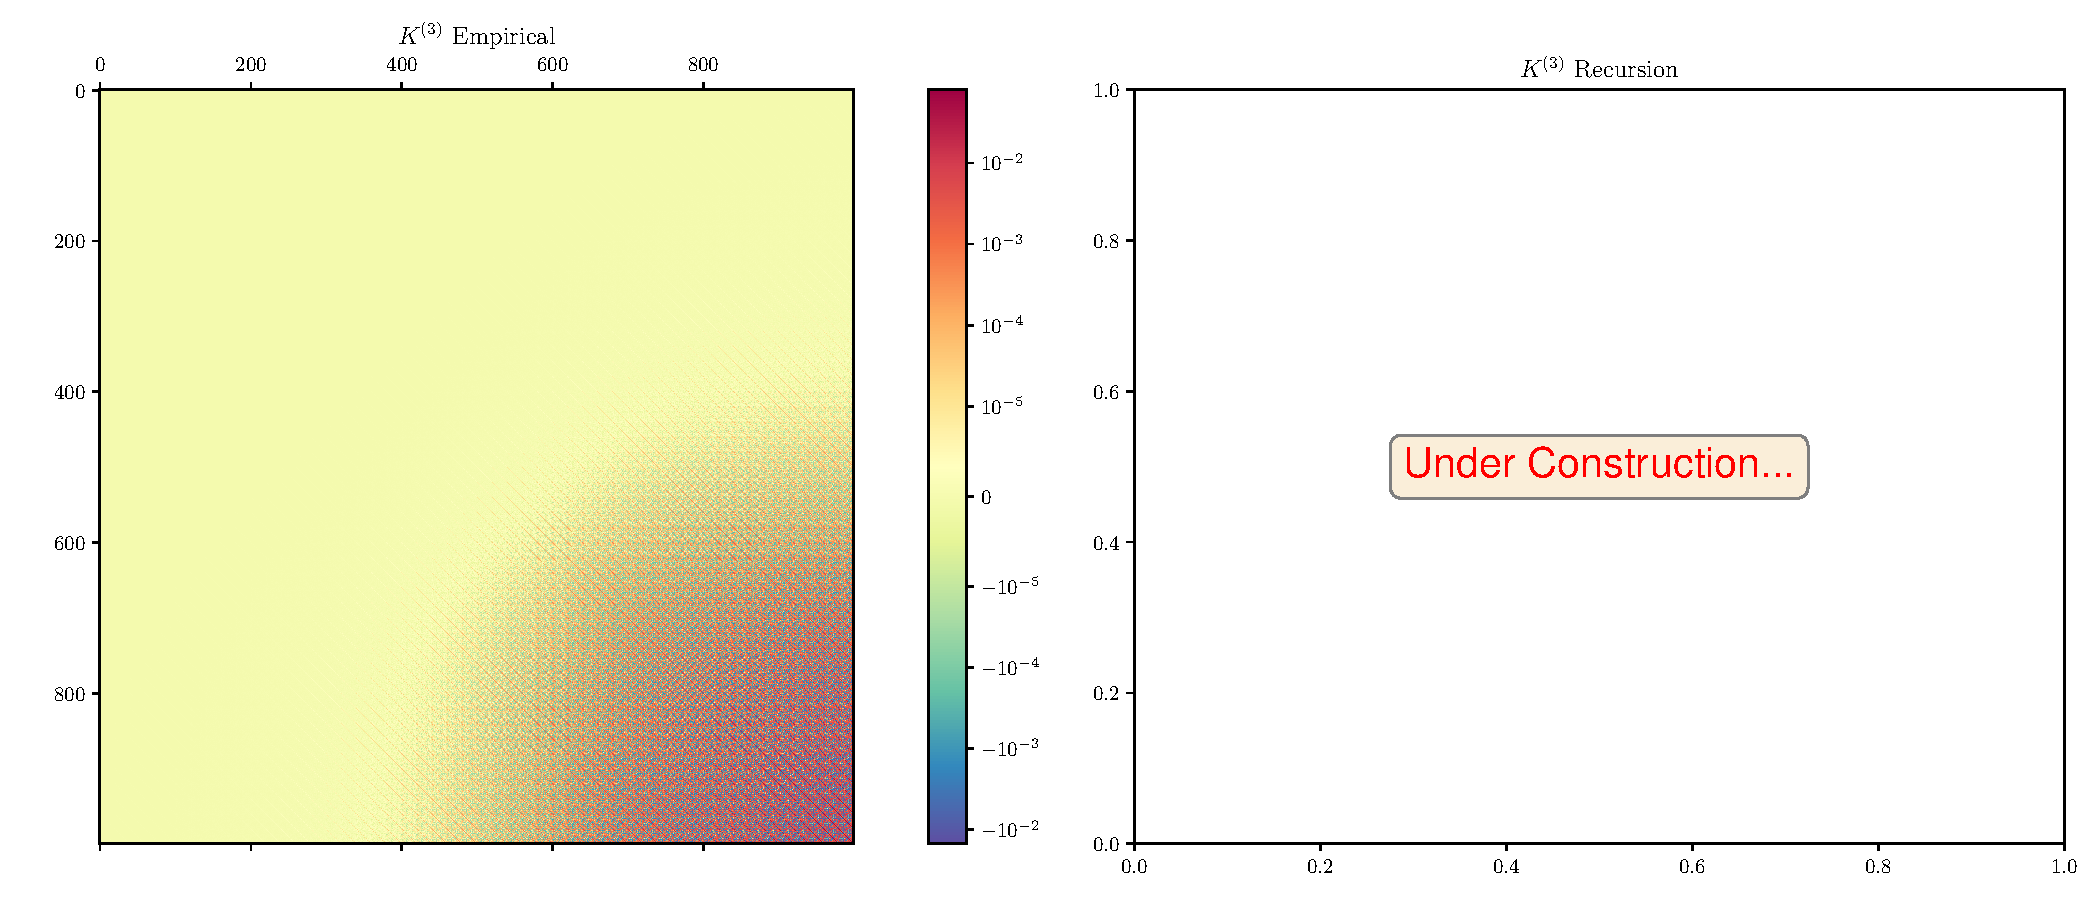
\includegraphics[scale=0.4]{figs/K3_correlations.pdf}
    \caption{Same as Fig.~\ref{Fig:KRecursionOne}, but for the second (top) and third (bottom) layers of the
    NNPDF architecture.
    \ac{Here the four indices of the covariance $K_{i_1i_2, \alpha_1\alpha_2}$ are flattened into
    two indices for the sake of graphical representation. Maybe we should group the labels into groups of
    $N_{\rm grid}$ ticks on the axes.}
    \label{Fig:KRecursionTwo}
    }
\end{figure}

As a consequence of the symmetry of the probability distribution, the mean value of the fields at
initialization needs to vanish, while their variance at each point $x_\alpha$ is given by the
diagonal matrix elements of $K^{(\ell)}$. The central value and the variance of the
parametrized singlet ($\Sigma$) and gluon ($g$) at initialization are shown in
Fig.~\ref{fig:SingletGluonInit} for an ensemble of $\nreps=100$. The central value is computed as
discussed above in Eq.~\eqref{eq:ReplicaEnsemble},
\begin{align}
    \label{eq:MeanValAtInit}
    \bar{f}_{i\alpha} = \bar{f}_{i}(x_\alpha) = \frac{1}{\nreps} \sum_{k=1}^{\nreps} f^{(k)}_i(x_\alpha)\, ,
\end{align}
and the variance $\sigma^2_{i\alpha}$ is computed using the same formula with
\begin{align}
    \label{eq:VarAtInit}
    O(f) = \frac{\nreps}{\nreps-1} \left(f_i(x_\alpha) - \bar{f}_{i}(x_\alpha)\right)^2\, .
\end{align}

\begin{figure}
    \centering
    
\includegraphics[scale=0.5]{plots/UoECentredLogo282v1160215.png}
    \caption{\ldd{Plot of replicas at init}}        
    \label{fig:SingletGluonInit} 
\end{figure}

\ldd{List of plots that we still need to do:
comparison analytical vs empirical, 
comparison analytical vs Gaussian processes}

\paragraph{Dependence on the architecture.}
Having analytical expressions for the variance at initialization allows us to investigate the
impact of the NN architecture on the prior that is imposed on the PDFs. Iterating
Eq.~\eqref{eq:RecursionForK} yields the covariance at initialization for various depths.
Do we get something interesting? worth mentioning?

\ldd{We should also look at the recursion relations with other activations. Again, check whether we
get something interesting...}

\FloatBarrier
